
\section{Case study: dynamical core}\label{sec:case1}

Our first case study focuses on CAM's spectral element dynamical core, known as HOMME (High-Order Method Modeling Environment) \cite{dennis:2012}, which is the default dynamical core for CAM for very high $1/4^\circ$ resolution simulations.  We focus on HOMME
because the dynamical core can consume 30-88\% of the total cost of the CAM and is particularly influential in the overall scalability of CAM and,  therefore, CESM (e.g., {\color{red}CITATION}).  We first provide more information on the HOMME dynamical core and then detail several modifications aimed at exascale.

\subsection{Algorithm details}

HOMME uses a cubed-sphere topology where each face of the cube is projected onto a sphere to generate a global computational grid.  HOMME uses a spectral element method to discretize in the horizontal and a finite difference approximation \cite{simmons:1981} in the vertical.  A continuous Galerkin finite-element method \cite{taylor:1997} is used for the spectral element method. The integrals used in the Galerkin formulation are computed from a Gauss-Lobatto quadrature rule within each element.  HOMME decomposes each time-step into components and the equation, for a compressible fluid with hydrostatic and a shallow water approximations, can be written in terms of a vector $U$ containing the prognostic state variables (velocity, temperature, and surface pressure) as: $dU/dt = F + D + A + T + R$, where $F$ represents the forcing from physics, $D$ the dissipation, $A$ the dynamics from the primitive equations, $T$ the tracer advection, and $R$ the vertical remapping of the mass and momentum variables. A diagram of the overall computational flow of the HOMME algorithm is provided in Figure \ref{fig:homme-alg}.

HOMME solves these equations in a time-split fully-explicit form. For time-steps involving the forcing ($F$) and dissipation ($D$) terms, a forward Euler time- scheme is used. The dynamics ($A$) and tracer advection ($T$) are computed using an N-stage Runge-Kutta time-scheme. The dynamics ($A$) computes the primitive equations prognostic variables. The tracer advection ($T$), is based on a finite-volume algorithm and advances the specific humidity, liquid water, ice variables, and additional tracer constituents. For advection, a vertical Lagrangian approach used \cite{lin:2004} where the horizontal advection on Lagrangian vertical levels is followed by remapping (R) the mass and momentum variables back to the reference vertical levels at the end of the time-step.

\begin{figure}[tbp]
 \begin{center}
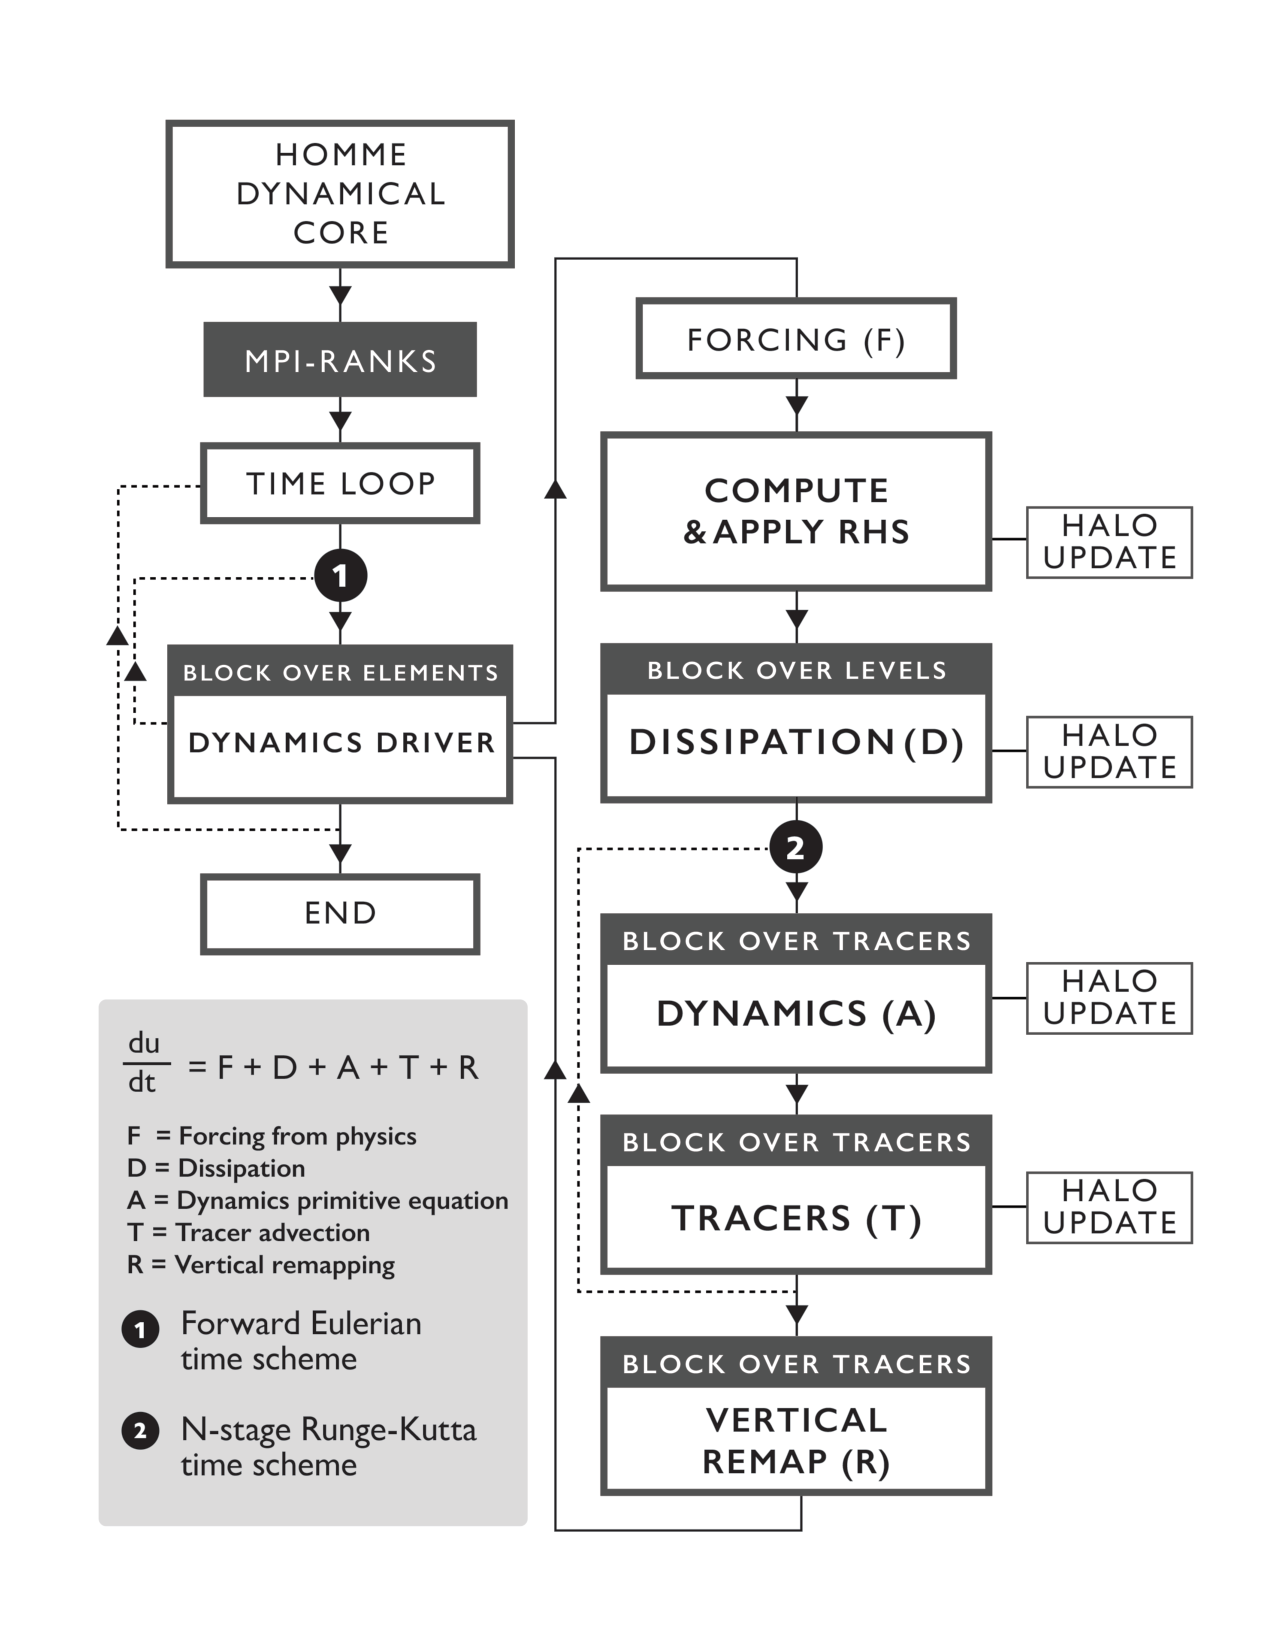
\includegraphics[width=12.0cm]{figures/HOMME-v01.pdf}
\end{center}
\caption{The computational phases within HOMME - {\color{red} how does this represent the flow and the new modifications?}.}
\label{fig:homme-alg}
\end{figure}

As with the rest of CESM, the HOMME dynamical core is written in FORTRAN 90 and utilizes a hybrid (MPI-OpenMP) programming model.  The resolution of HOMME's cubed-sphere computational grid is indicated by the number of spectral elements on a side of a cube ($ne$). In particular, each side of the cubed-sphere computational grid is tiled with $ne \times ne$ spectral elements, resulting in a total number of spectral elements of $nelem = 6 \times ne \times ne$, where {\em nelem} is the total number of elements.  For reference, CAM is typically run in production at $ne=30$, which roughly corresponds to 1-degree resolution with grid points approximately every 100 km.  High resolution simulations at quarter-degree resolution (i.e., $ne=120$) with grid points approximately every 25 km, such as the simulation in \cite{small2014}, typically require very large core counts for an extended periods of time.  
The spectral elements are statically partitioning during initialization across either MPI tasks or OpenMP threads. 
Note that the simulation in \cite{small2014}, corresponding to $ne=120$ and $nelem=86,600$, used a total of 21,600 hardware cores which resulted in the assignment of 4 elements per core.
The performance of HOMME is strongly influenced by the number of spectral elements allocated to each hardware core, and historically, while it was technically possible to scale HOMME to core counts equal to the number of spectral elements {\em nelem} it was, in practice, cost prohibitive.


[{\color{red} What CESM/CAM/HOMME version(s)?.}]


\subsection{Revised parallelization strategy}

[{\color{red} still needs some work.}]

We begin with the extensive code changes needed to allow higher levels of parallelism.
As mentioned in the previous subsection, the original HOMME parallelization scheme
partitioned over elements at a  high level and loops at lower-levels.  This strategy fundamentally limited the number of cores (MPI tasks?)to be at most equal to the number of 
spectral elements {\em nelem}. {\color{red} Suggest saying more on limits here so that the improvements below make more sense.}


The revised scheme uses the same high-level parallelization over elements, however, the lower-loop level parallelization has been replaced with a high-level parallelization over the vertical level and tracers dimensions. The dimension chosen to parallelize is dependent on the region (dynamics, tracer advection, dissipation, or vertical remapping) of the code.
The revised scheme has several improvements over the original approach. These improvements include: a significant reduction in the number of threaded regions created; allows a greater number of threads to be assigned; allows replacement of MPI-Ranks with OpenMP threads which reduces the total MPI communication; provides greater flexibility in determining where the threads are assigned in the regions of the code; simplifies the scoping of variables in the parallel region as variables local to the routines, inside the parallel region, are private; minimizes wastage of thread resources as the parallelized over the vertical level and tracer blocks do not overlap so threads can be shared between these regions

The revised parallelization structure of HOMME is shown in Figure \ref{fig:homme-alg}. Elements within the global domain are initially assigned with MPI-Ranks. Within the time loop, we maintain the original parallel structure over elements. The dynamics driver calls the dynamics, tracers, dissipation, and vertical remapping modules. These are parallelized over tracers or vertical levels; the blocking scheme chosen was dependent on the parallelism available in the module. In the dynamics, tracer and vertical remap modules, the code is blocked over tracers and in the dissipation module the code is blocked over the vertical levels. The only component module where we have maintained the original loop level-parallelism is in the 'compute\_and\_apply\_rhs' module as dependencies in the vertical prevent blocking over levels. 
The code changes needed to implement the revised parallelization strategy were extensive. However, they could be made systematically which simplified the implementation process. Invocation of the blocked regions dynamics, tracers, dissipation, and vertical remap can be understood with a simple example:

\begin{verbatim}
  call omp_nested(.true.)
  !$OMP PARALLEL NUM_THREADS (num_threads_region) & 
  !$OMP& DEFAULT(SHARED), PRIVATE(hybrid_region)
    hybridreg = config_thread_region(hybrid, regtype)
    call foo (hybridreg, ...)
  !$OMP END PARALLEL
  call omp_nested(.false.)

  subroutine foo (hybridreg, ...)
      call get_loop_ranges (hybridreg, lbeg, lend)
  end subroutine foo	

\end{verbatim}

Where the variable 'regtype' is name of the parallelism implemented in the module (element, level or tracer); 'hybridreg' is a derived type that contains the mapping from the thread number to the starting and ending indices for each 'regtype'; '��`num\_threads\_region"�� is the number of threads assigned in the 'regtype'.

The declaration of the number of MPI-Ranks and OpenMP threads for the elements, tracer, and vertical is performed at run-time. The design of HOMME with inner indices (np,np) are known at compile-time which allows the compiler to generate efficient vectorized code with the limitations described in Section {\color{red} ??}. The specification of the number of levels and tracers are made at run-time without impacting performance.

\subsection{Single-core optimization}

[{\color{red} better transition here}] A second aspect of HOMME that clearly needed optimizing
based on performance analysis was ...


The single-core performance optimizations implemented included improving: vectorization, data locality, minimize computations, and compile-time specifications for loop and array bounds \cite{henderson:2015}. Each of these techniques has contributed to the overall single-core performance improvements in the code. The overall results of these optimizations are discussed in Section \ref{sec:homme-results}.

The software design approach used in HOMME inhibited some optimizations techniques. The inner-loops, details of which are described below are written as (np,np) were collapsed and vectorized, but the loop index was not linearized as the compiler generates gather and scatters and not unit stride loads and stores. As the number of vector-registers on the AVX2 and AVX-512 has increased linearizion of the loop indices to generate longer vectors becomes of significant importance to performance.

The use of function statements throughout the code does impact performance. When inlining was forced with a compiler directive, the compiler did inline the function, however, the code generated was not as efficient as when the function was manually inlined. This was the result, not of the data copy across the function boundary, but from the optimizer performing more aggressive loop optimizations for the manually inlined code.

Finally, the compiler reports, provide information on details of alignment of data for each vectorized loop. Where the data was not aligned, the compiler flag (-align arraybyte64) and the OpenMP aligned directive does force data alignment. However, the directive is cumbersome to create for complex loop as all unaligned variables need to be defined in the aligned list. This creates a maintainability issue; there are also issues when alignment is forced as it can lead to incorrect answers. For these reasons, we have avoided forcing data alignment in the code.

\subsection{Data and loop structures}


[{\color{red} better transition here}] Next, we looked at .... because ....

The data structures are dynamically allocated and maintain a global index within each MPI-Rank.  Allocation of a generalized variable has the following ordering convention:

\begin{verbatim}
   variable_name[np,np,nlevel,ntracer,nelem]
\end{verbatim}

Where np*np is the number of points in the quadrature grid, nlevel is the number oj vertical layers, ntracer the number of tracer variables, and nelem the number of elements per MPI-Rank.

At the highest level in the code, we have the loop structure:

\begin{verbatim}
do ie=nets,nete
    call dynamics_driver()
enddo
\end{verbatim}

Where nets and nete are the starting and ending number of the elements in each MPI-Rank. The loop structure within the dissipation, dynamics, tracers, and vertical remapping modules are written as:

\begin{verbatim}
do q=qbeg,qend
 do k=kbeg,kend
    variable_name(1:np,1:np,k,q,ie) = ...
  enddo
 enddo
\end{verbatim}

Where the element index 'ie' is defined above, 'kbeg, kend, qbeg, and qend' loop ranges are defined from 'get\_loop\_ranges' for the vertical levels and traces respectively and are evaluated for each thread number within the parallel region. The algorithm used to create these loop bounds is designed to minimize the load imbalance in the work that each thread performs. For the dimensions that are not blocked within the parallel region, they are simply defined as '1:nlevel and 1:ntracer'.

Prior to the blocked implementation, the loop bounds in the code, were written:

\begin{verbatim}
  do q=1,ntracer
     do k=1,nlevel
        variable_name(1:np,1:np,k,q,ie) = ...
     enddo
  enddo
\end{verbatim}

A significant number of code changes were needed to create the blocked implementation. However, no changes were needed for the element region type as this was already supported in the original dynamical driver. The memory allocation for the variables remained unchanged. Changes were made to the halo-update communication routines so they were thread safe within the blocked levels, and tracer regions.


\subsection{Other modifications}

Clearly HOMME has received much of our attention and many modifications have been implemented to improve its performance for exascale. Here we note that in addition to those improvements detailed in the subsequent three subsections, additional modifications contribute to the improved performance shown in Section \ref{sec:bench}.  For brevity, we simply list
the additional modifications here:

{\color{red} Fix bullets so that they are two or three sentences long - so slightly more info for reader. Remove any already discussed above.}
\begin{itemize}
   \item Threading memory copy in boundary exchange [PARALLEL]
   \item Restructured data-structures for vectorization [SERIAL]
   \item Rewrote message passing library/specialized communication operators [PARALLEL]
   \item Rearranged calculations in euler\_step for cache reuse [SERIAL]
   \item Reduced number of divides [SERIAL]
   \item Restructured and aligned for better vectorization [SERIAL]
   \item Rewrote and optimized limiter [SERIAL]
   \item Redesigned the OpenMP threading [PARALLEL]
\end{itemize}


\subsection{Benchmarking results}\label{sec:bench}

\input homme.tex